\section{Design}

\subsection{System-level design}
The complete system will consist of energy harvesting source, energy storage for times when harvested energy is not available, AC/DC and DC/DC converters for maintaining required voltage levels in different blocks of system, accelerometer for measuring the accleration in tyre and bluetooth/microcontroller module for transmitting data from acceleromoter. Figure \ref{system_blog_diagram} shows the power and data flow between subsections of system. 


\begin{figure}[htb]
\begin{center}
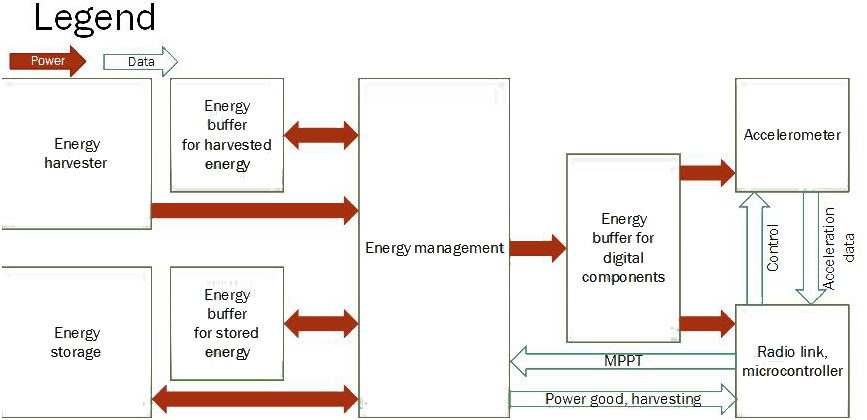
\includegraphics[height=6cm]{images/system_block_diagram.jpg}
\end{center}
\caption{\label{system_blog_diagram} Block diagram of complete system.}
\label{liitekuva}
\end{figure}


\subsection{Power requirements of a system}
The sensor system will be in three distinct states. One is sleeping, conserving power as much as possible while car is not moving.
Second state is measuring, when the radio connection is off but electronics are active and gathering data.
Third state is transmitting, when the data is relayed to drive computer in car.

Energy and power consumption are estimated by reviewing a few suitable components and their power requirements. 
Energy management is handled by a specialized integrated circuit (IC), for example LTC3331 \cite{Technology}.

Communication is handled by a Bluetooth-low energy (BLE) module, which contains a general-purpose microcontroller for application flow control.
We use BLE113 \cite{Bluegiga2013} as an example of such module.

Finally there is an accelerometer which is used for gathering data out of the system, ADXL375 \cite{ADXLDatasheet} is used as an example. ADXL is a low-power digital accelerometer with dynamic range of 200g. Table \ref{power_consumption_table}  summarizes the estimated power requirement of each subsection of system. System level voltage is selected to be 2.5 V, as that is lowest voltage which LTC3331 can supply and allows all devices to function. Lowest possible voltage is selected to reduce the power draw.

\begin{table}[htb]
\caption{\label{power_consumption_table} Current and power consumption of system at different activity levels.}
\begin{center}
\fbox{
\begin{tabular}{l l r r}
\textbf{Device}		& \textbf{Sleep} 	& \textbf{Monitoring}	& \textbf{Communicating}\\ \hline
LTC3331			& 0.2 $\mu A$		& 80 $\mu A$ 		& 16 250 $\mu A$ 		\\ \hline
BLE113			& 0.9 $\mu A$ 		& 275 $\mu A$ 		& 26 000 $\mu A$	\\ \hline 
ADXL375			& 0.1 $\mu A$ 		& 140 $\mu A$ 		& 140 $\mu A$		\\ \hline \hline
\textbf{Total power}	& 3   $\mu W$		& 1 200 $\mu W$		& 110 000 $\mu W$	
\end{tabular}
}
\end{center}
\end{table}

Power consumption grows by orders of magnitude when the activity is stepped up to next level. Therefore it's important to keep the system in sleep whenever possible, for example when the car is parked and wake up only periodically to check if movement has started. Monitoring starts once car is moving, and device will send brief pulses over the radio link when necessary.

Battery manager power draw is estimated by calculating required power to supply the rest of the circuit at 80 \% efficiency.


\subsection{Electromagnetical harvester design}
\subsubsection{Basics of electromagnetical vibration harvester}
Electromagnetic harvesters utilise vibration to move a magnet inside a coil. The movement of a magnet causes a changing magnetic field, which gets coupled to coil. Coil opposes the change in magnetic field by inducing electrical current in device. {\color{red} cite} A device could be built with a spring-loaded magnet to balance out the static acceleration of a tyre. An added bonus to spring loaded mechanism would be the utilisation of resonant frequency of the spring-mass system: as the system gets a shock, some of the energy would be in correct frequency range to make the magnet oscillate inside coil allowing generation of energy until next shock. The coil will also function  as a dampener to system, so no extra dampening is required. Primary concern is the survivability of a magnet in an environment with heavy shocks and vibration. 

A theoretical design of linear generator was made. Most common generator designs use a rotating magnet inside coils to generate alternating current. As the mechanical apparatus for converting the linear accelerations inside tire to rotational movement would add to complexity and cost of the tire, generator is design to use the linear motion as the power source.

Basic principle of operation is similar to traditional rotational generator. A moving magnet creates alternating magnetic field which is coupled to coiled conductors. The conductors oppose this change of magnetic field by inducing an electrical current across their ends. The design can have multiple phases and poles. Multiple phase designs can be made smaller and lighter at the expense of more complex control circuitry. {\color{red} cite}. 

Adding poles to design increases the output voltage {\color{red} cite a study of multi-pole} and frequency, but having a small airgap between the coils and magnets becomes critical to maintain efficiency of the generator. 

A simulink model was built to verify feasibility of the linear generator. The model included real acceleration data from previous studies made by {\color{red} cite} and a model of generator as well as a simplified capacitive-resistive load. There is an abundance of previous work done on simulating linear generators  {\color{red} cite}, however a simplified model was used at this stage to get a proof-of-concept level generator. Further work remains in optimizing the design in terms of size, mass, power output, usable speed range, cost and long-term reliability.

First design decision was whether to use a moving magnet or moving coil type of a design. Moving coil designs tend to have lighter moving parts which is a very important feature in high-power designs where mass of the generator is large. On the other hand, moving coil require flying leads  {\color{red} cite development of a moving magnet linear}.  which is a long-term reliability concern  {\color{red} cite linear electric actuators and generators}.  {\color{red} cite book Boldea, Nasar Linear electric actuators and generators p 203}. conclude that moving coil designs aren't practically interesting, so the design is focused on moving magnet generator. 

A rough model for designing initial prototypes was done previously by  {\color{red} cite backpack harvester}. As the work verified the model experimentally and found the model to be reasonably accurate, it was adapted to form basis of linear generator model. The model can account for most of the key design parameters. 

\begin{table}[htb]
%% Taulukon teksti
\caption{\label{parameters_of_lg} Effect of parameters of generator}
\begin{center}
\fbox{
\begin{tabular}{l l l}
\textbf{Parameter}		& \textbf{Increasing} 		& \textbf{Decreasing}	\\ \hline
Number of turns in generator	& Higher voltage		& Smaller size, less wiring resistance 		\\ \hline
Number of poles			& Increased frequency		& Decreased frequency	\\ \hline
Distance between poles  	& More space for wiring 	& Higher voltage, smaller size	\\ \hline
Wiring radius		  	& More power			& Smaller length of wiring 	\\ \hline
Magnetic field strength  	& Increased power 		& Smaller magnets 		\\ \hline
Wire diameter		  	& Decreased wiring resistance 	& More turns in same space 	\\ \hline
Gap to wiring			& Stronger side walls		& Incresed efficiency 
\end{tabular}
}
\end{center}
\end{table}

Energy harvester designs often use several poles to increase the frequency of the power output {\color{red}cite}. This increased frequency allows to use smaller energy storage components such as capacitors to keep the device powered until next cycle. The characteristics of the tyre make this point a moot, as energy is available once per revolution of the tire when generator contacts the ground and when the contact ends. Any energy storage device has to maintain power until the next cycle, and no increase of the frequency while generator is in contact can alleviate that. Therefore number of poles is minimized to reduce complexity. Pole number is selected as two, so there is one negative and one positive pole. 

There are two different approaches to generator structure. One is magnets inside, and coils on the outer rim of the generator. Other is to use ring magnets on the outer rim and have the coils on the inside. Both methods have their advantages: Having magnets on the outside allows larger and therefore stronger magnets and creates horizontal support for the magnets as they slide along the shaft. Having coils on the outside increases wiring radius which results in greater power if other parameters are held equal. In-depth study of both concepts is done to select optimal structure for generator. 

The height of the generator is constrained at  {\color{yellow} confirm} 45 mm. Initially the height of {\color{gray} the} generator was selected to be 35-40 mm to leave some margin while still being as tall as possible. Lower weight is desirable to avoid unbalancing the tyre, but there is no specific absolute maximum mass for the device. 

A method to counter the centripetal acceleration is needed to avoid jamming the magnet on the bottom of the generator. Ideally, such method would always balance the magnet in the middle of generator against any external constant force, but active control is not achievable without adding to complexity and power consumption of the generator itself. Passive negative feedback method has to be used instead. 

Springs are often chosen {\color{red} cite few sources} to balance the magnets, but as the centripetal acceleration grows exponentially with the speed of the car, any linear spring would be usable only for very limited range of speeds. Non-linear conical springs which have the added benefit of compressing into very small height are available.

Another approach would be to use two additional magnets fixed to top and bottom of the generator in repulsive configuration. Force between magnets is inversely propotional to fourth power of the distance {\color{red} cite}, which leads to a strong negative feedback on the position of the magnet. 

Magnetic floating is very attaractive solution, as magnets can be very thin and they do not wear out with aging. On the other hand, any imbalance in the magnets result in torgue which causes increased friction. {\color{yellow} picture?} This issue is further aggravated in designs where shape of the generator shaft is not a smooth cylinder. Therefore the design should have any grooves filled with suitable epoxy and the shaft should be sanded or turned to final diameter to ensure smooth sliding across the length of shaft.

\subsubsection{Analytical model of electromagnetical vibration harvester}
A common starting point for analysis of linear generator is to model the mechanical domain as Mass-Spring-Dampener system decipted in figure \ref{MSD}. A mass "floats" in system, a spring balances the mass towards balance and a damper represents frictional forces opposing any movement of mass. 

\begin{figure}[htb]
\begin{center}
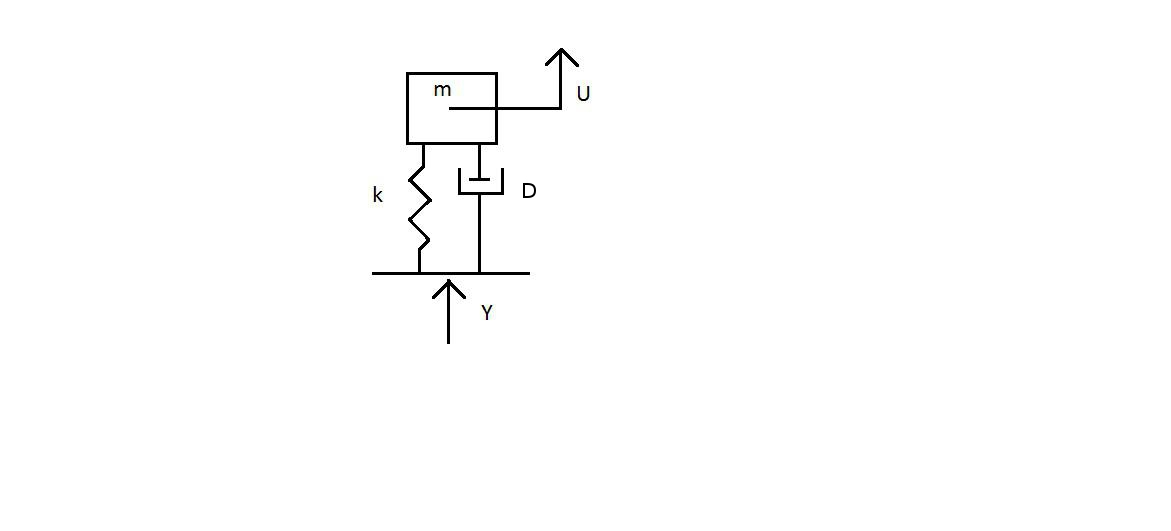
\includegraphics[height=6cm]{images/own_dwg/MSD.jpg}
\end{center}
\caption{\label{MSD} Mass-spring-damper system.}
\end{figure}

Input Y is the force applied to the base of system, output U is the position of mass block relative to "zero". Zero is usually set to point where mass settles when no input, including gravity, is applied to system. Paramters m, B, and k are mass, damping constant and spring constant of system, respectively. Input-output-equation in time domain can be written as: 

\begin{equation}\label{eq:MSD_basic}
  m * \ddot{U}(t) + B * \dot{U}(t) + k * U(t) = Y(t). 
\end{equation}

As the force $ Y(t) $ is defined as $ Y(t) = m*a(t) $, and the acceleration $ a(t)$ can be considered constant regardless of any reasonable mass $ m $ of system, equation \eqref{eq:MSD_basic} can be written as:

\begin{equation}\label{eq:MSD_acceleration}
 \ddot{U}(t) + \frac{B * \dot{U}(t)}{m} + \frac{k * U(t)}{m} = a(t). 
\end{equation}

This form is convenient for analysis, as the acceleration measurements from previous research are available and they represent real-world values. Mass m can be considered constant, as the system does not exchange matter with surrounding environment. As magnetic suspension was selected, the paramter k cannot be considered as a constant, but rather a function of mass position $k(U)$. Centripetal force can be considered as a constant DC-component of function $Y(t)$, and is not included in analysis of function $k(U)$. According to D. Amrani \cite{Amrani2015} force between two magnets can be approximated as

\begin{equation}\label{eq:magnetic_force}
  F(x) = \frac{3 \mu_0 m_1 m_2}{2 \pi} * \frac{1}{x^4},
\end{equation}

where $F(x)$ is force as a function of distance x between magnets, $\mu_0$ is the permeability of vacuum, $ m_1 $ and $ m_2 $ are magnetic dipole moments of magnets under examination. This equation is only valid when x >> h, where h is thickness of the magnet. As two magnets are used to suspend the rotor magnet, total force acting on mass becomes 

\begin{equation}\label{eq:magnetic_force_middle}
  F(x) = \frac{3 \mu_0 m_r m_l}{2 \pi} * \frac{1}{(x_0+x)^4} - \frac{3 \mu_0 m_r m_u}{2 \pi} * \frac{1}{(x_0-x)^4},
\end{equation}

where $m_l, m_u, m_r$ are magnetic dipole moments of lower suspending magnet, upper suspending magnet, and rotor magnet. $x_0$ is the distance to middle point of generator and $x$ is the displacement of rotor magnet from aforementioned middle point, positive direction being upwards. Figure {\color{red}draw figure} shows the system.

Regrettably, the expression \eqref{eq:magnetic_force_middle} is very inaccurate for magnets where diameter is large compared to thickness of magnet, and the problems are compounded when distance between magnets is small. Therefore final design should be optimized using measurement data or finite element analysis (FEA) for determining $k(U)$. 

Damping parameter $B$ is likevise a function electromagnetic force acting on magnet, friction between magnet and stator and pneumatic damping caused by compression of air in generator. Tornincase et al. \cite{Tornincasa2012} divided this damping parameter into three distinct terms to account for these different physical phenomena in damping. Let us call them $B_{emf}, B_{friction}, and B_{air}$, respectively. $B_{emf}$ represents power extracted from the system into electrical current, it can be written as:

\begin{equation}\label{eq:emf_force_middle}
  \varepsilon = 
  B_{emf} = -n * 
\end{equation}

\subsection{Piezoelectric design}
A previous work by 

\subsection{Hybrid design}

\subsection{Electrical design}
The analog sections of circuit were simulated using LTSpice IV {\color{red} reference}. Accelerometer and bluetooth module were modeled as parallel current sinks which took energy from the circuit in pulses. Energy harvesting was simulated as a high.impedance AC voltage source. 
Battery was modelled as a voltage source with high-value capacitor and low-value resistor in series.

\subsection{Materials for the harvester}
Material for the shaft has a few requirements. It has to have at least as good temperature characteristics as the magnet being used and it must be hard enough to not deform under impacts. Low friction coefficient is desirable as this leads to smaller losses, and long time durability under wear is of course desired. Being lightweight and easily machinable are also desired characteristics. As the generator is small, volumetric cost of the material is of little concern. For the electro-magnetic generator design material also has to be non-ferromagnetic {\color{red} verify?}. Table {\color{yellow} refer?} has comparison of different materials considered for the application.

\begin{table}[htb]
%% Taulukon teksti
\caption{\label{parameters_of_materials} Materials for the shaft of generator}
\begin{center}
\fbox{
\begin{tabular}{l l l l l l}
\textbf{Material}& 
\textbf{Hardness \cite{PlasticsInternational2015}}& 
\textbf{Friction \cite{Etra}} & 
\textbf{Durability \cite{Etra}} & 
\textbf{Temperature \cite{Etra}}\\ \hline
PTFE(Teflon)      & Very low   & Lowest                      & Lowest    & -190... + 250 \degree C \\ \hline
Polycarbonate     & Very high  & High  \cite{Goodfellow}     & -         & -60... + 125 \degree C \\ \hline
PA 6 (Nylon)      & Low        & Medium                      & High      & -40... + 80 \degree C  \\ \hline
Oil-infused Nylon & Low        & Very low                    & Very high & -20... + 105 \degree C \\ \hline
Acryllic          & High       & -                           & -         & -40... + 70 \degree C \\ \hline
Polyacetal (POM C)& Medium     & Low                         & Low       & -50... + 105 \degree C \\ \hline
\end{tabular}
}
\end{center}
\end{table}


